\mysubsection{Sarah Häfele}{Aufbau}
Da die Installation aus mehreren Hardware- und Software-Komponenten besteht, soll hier eine kurze modellhafte Übersicht über den endgültigen Aufbau des Prototypen skizziert werden. Die darauf folgenden Kapitel gehen anschließend näher auf die einzelnen Komponenten ein. Der Prototyp der Installation wurde am 20.01.2015 im Rahmen des \textit{Tag der Medien} der Fakultät Digitale Medien aufgebaut und getestet. Auf zwei Ebenen wurden Gerätschaften installiert, damit die Besucher schon beim Eintreten mit akustischen und visuellen Reizen konfrontiert und zum Mitmachen bewegt wurden. Die zwei Grafiken zeigen das Erdgeschoss und den ersten Stock des Gebäudes.
\begin{figure}[h]
	\centering
		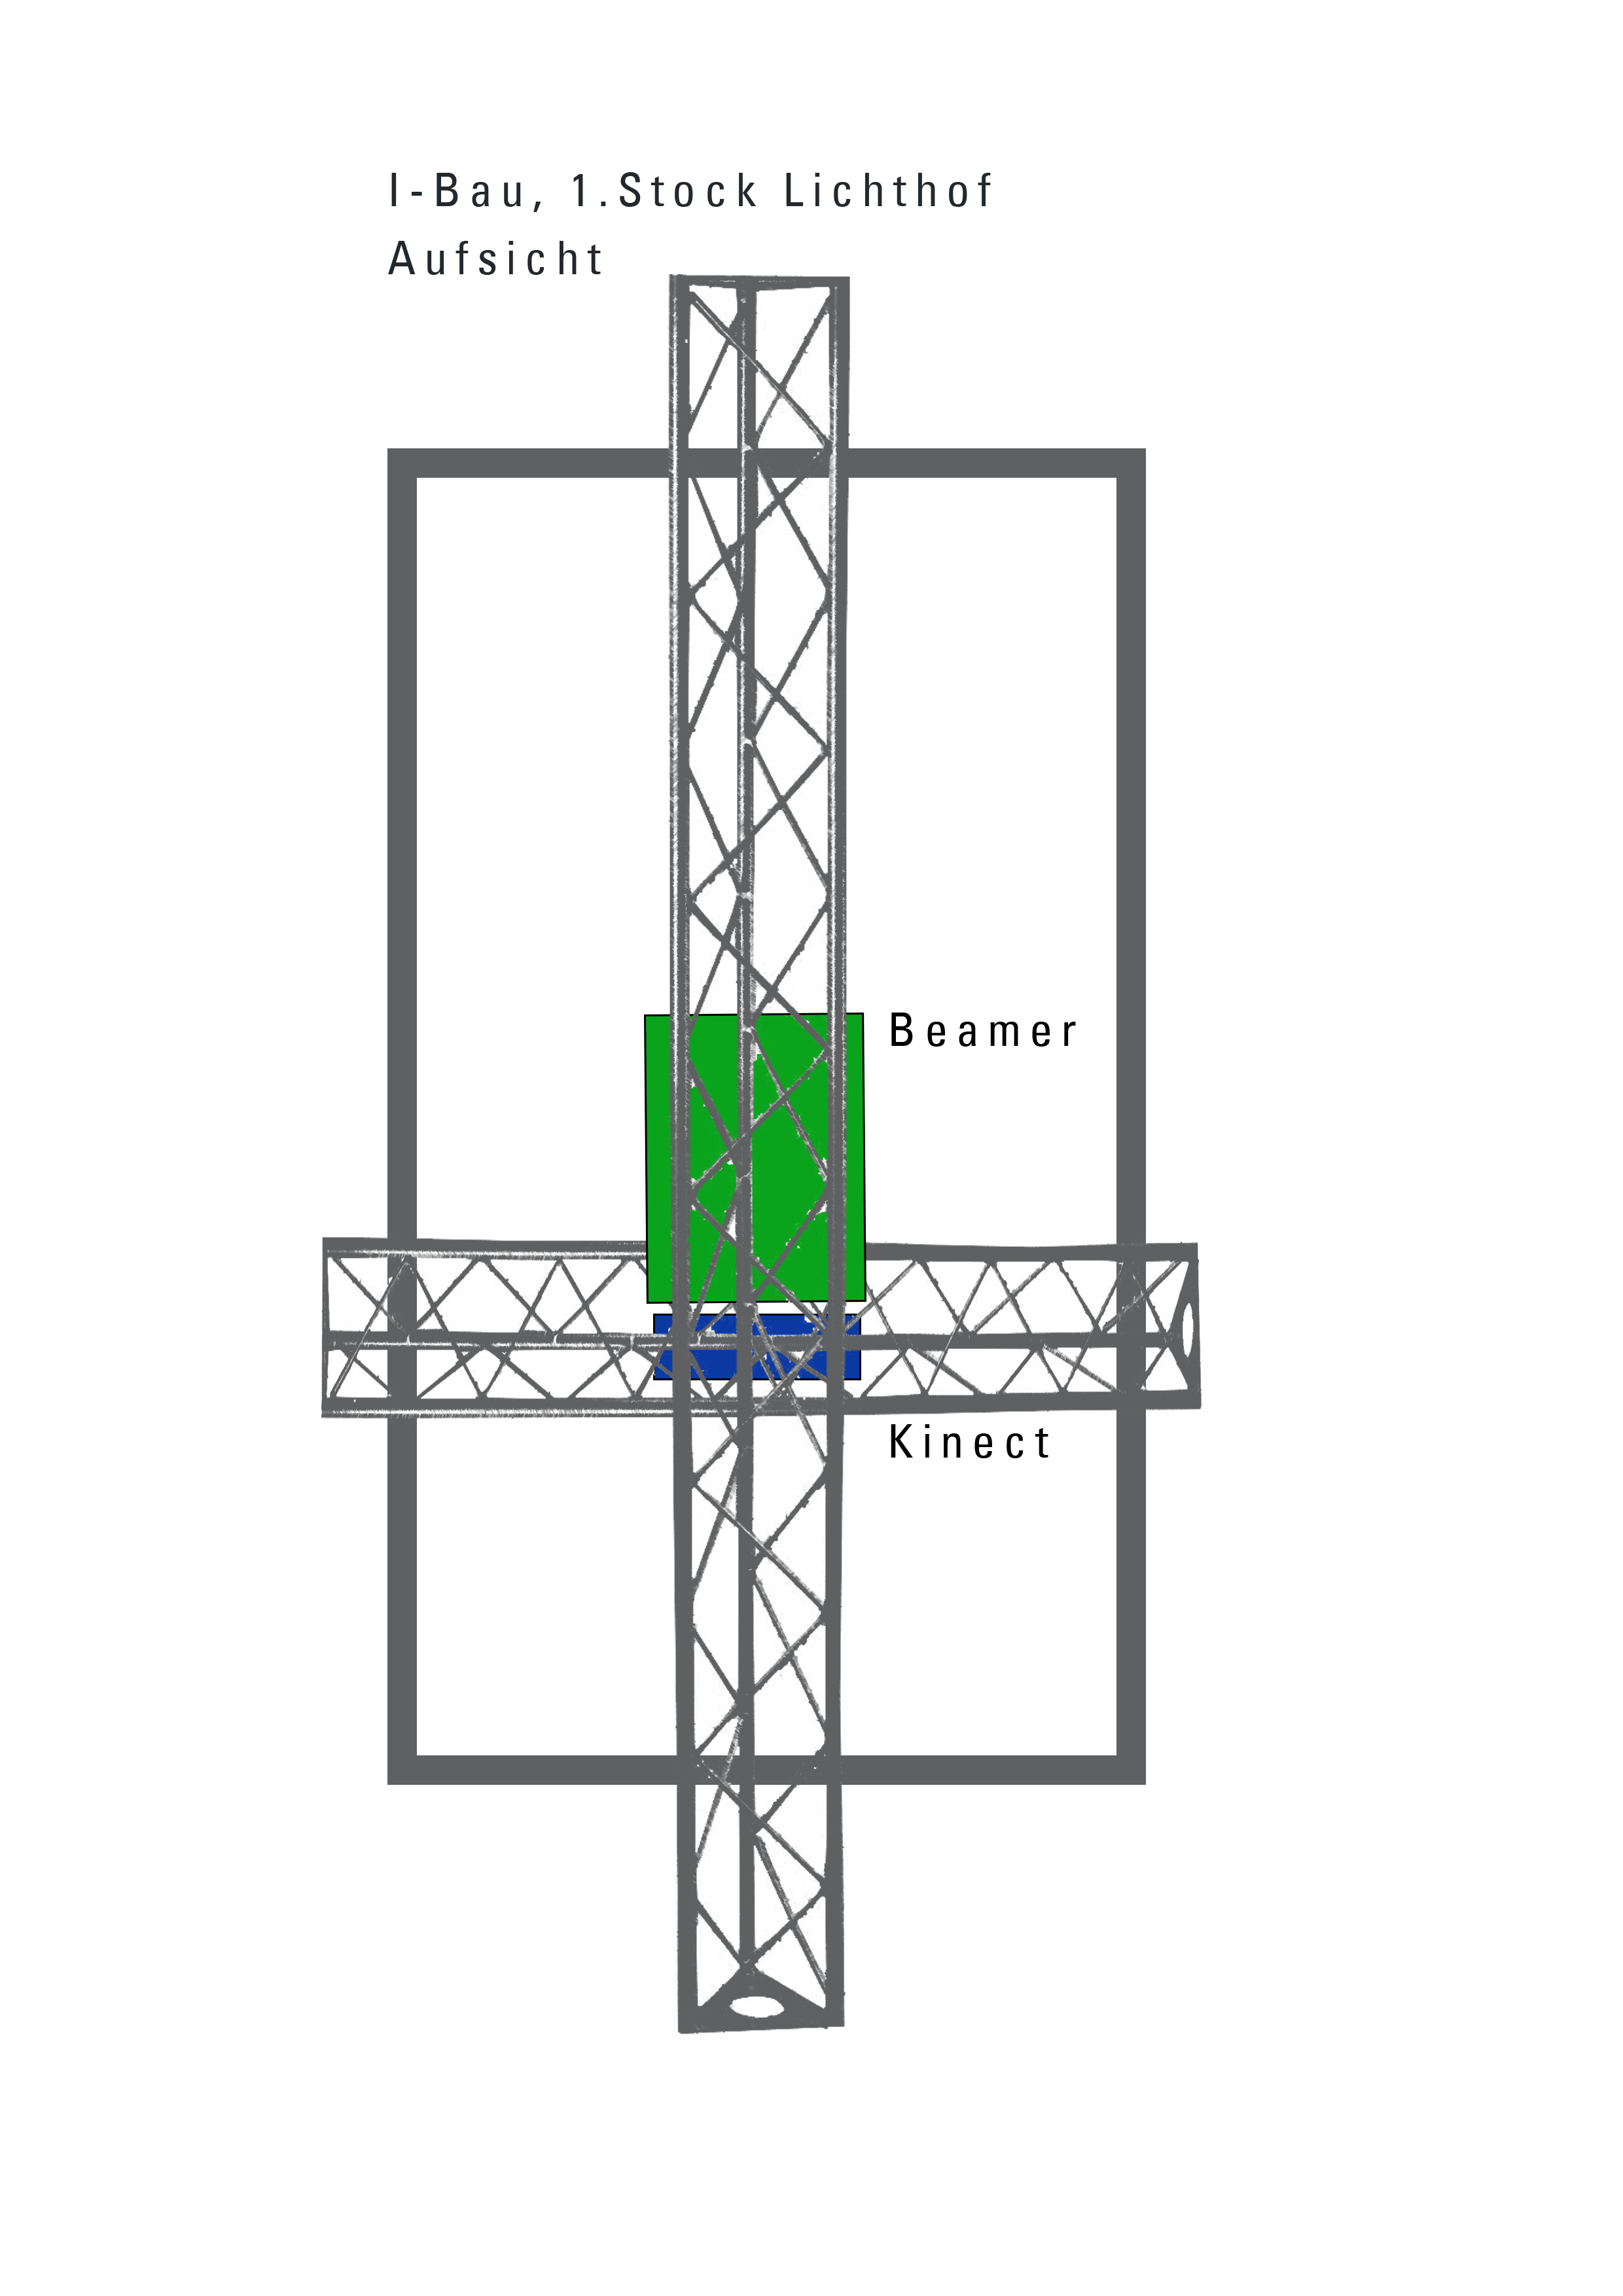
\includegraphics[width=0.90\textwidth]{images/ModelFirstFloor.png}
	\caption{Aufbau der Installation im 1.Stock des I-Baus}
	\label{fig:ModelFF}
\end{figure}

Im ersten Stockwerk hängt über dem Lichthof eine zwei Meter lange Traverse, getragen von zwei Stativen, in deren Mitte ein Epson EB-4950WU Beamer (in der Abbildung \autoref{fig:ModelFF} grün markiert) an einer speziell von der Werkstatt der Hochschule angefertigten Metallhalterung in das Erdgeschoss des Gebäudes strahlt. Der Beamer, eine Leihgabe des Kreismedienzentrums Villingen, kann mit seiner Farbhelligkeit von bis zu 4.500 Lumen und eine Auflösung von 1920 x 1200 Pixeln den dunklen Boden des I-Baus mühelos ausleuchten und ist zudem für längere Betriebszeiten ausgerichtet. Durch die erhöhte Stellung der Traversenstative hängt der Beamer sechs Meter über dem Erdgeschossboden. \\
Auf der Brüstung des Lichthofes liegt im 90° Winkel dazu eine ein Meter lange Traverse. Sie wird nicht ganz mittig zu der längeren Traverse ausgerichtet, damit die daran befestigte Microsoft Kinect (in der Abbildung in blau markiert) nicht das Bild des Beamers stört. Durch die direkte Anbringung auf dem Geländer des Lichthofes, hängt die Kinect zudem auf 4,5 Meter Höhe und kann so bequem die Bewegungen der im Erdgeschoss befindlichen Personen aufnehmen. 


PC --> software


